\documentclass[a4paper,9pt]{extarticle}

\title{cheat sheet}
\date{2016-03-09}

\usepackage{pew}

\begin{document}
\begin{multicols*}{2}

% COPYRIGHT
% 
% This is a summary of:
% Introduction to Linear Algebra for Science & Engineering
% by Daniel Norman and Dan Wolczuk
% ISBN 978-1-78434-351-4
%
% All rights belong to the authors - i don't own anything.
%
%
% CHAPTERS
%
% * **Euclidian vector spaces** – Chapter 1.1-1.5
% * **Systems of linear equations** – Chapters 2.1-2.3
% * **Matrices and linear mappings** – Chapters 3.1-3.5
% * **Vector spaces** – Chapter 4.1-4.6
% * **Determinants** – Chapter 5.1-5.4
% * **Eigenspaces** – Chapter 6.1-6.2
% * **ON-basis** – Chapters 7.1-7.3
% * **Spectral theorem and quadratic forms** – Chapters 8.1-8.2

% ================================================== %
% == Euclidean Vector Spaces  == %
% ================================================== %

\section{Euclidean Vector Spaces}
\subsection{Linear combination [1.1]}
\begin{equation} \label{1.1-1}
    \begin{split}
        \vec{v} & = \begin{bmatrix}v_1 \\ \vdots \\ v_n\end{bmatrix} 
            = v_1\begin{bmatrix}1 \\ \vdots \\ 0\end{bmatrix} + ... + 
            v_n\begin{bmatrix}0 \\ \vdots \\ 1\end{bmatrix}
            = v_1 \vec{e_1} + ... + v_n \vec{e_n}
    \end{split}
\end{equation}
Any vector can be written as a unique linear combination of the standard basis vectors.

% ================================================== %

\subsection{Vector equation of a line through point $P$ [1.1]}
\begin{equation} \label{1.1-2}
    \begin{split}
        \vec{x} & = \vec{p} + t \vec{d}, t \in \mathbb{R}
    \end{split}
\end{equation}

% ================================================== %

\subsection{Directed line segments [1.1]}
Denote the directed line segment from point $P$ to point $Q$ by $PQ$.
\begin{equation} \label{1.1-3}
    \begin{split}
        \vec{PQ} & = \vec{q} - \vec{p}
    \end{split}
\end{equation}
A directed line segment that starts at the origin is called the position vector of the point: $\vec{OP} = \vec{p}$.

% ================================================== %

\subsection{Entities [1.2]}
For all $\vec{w}, \vec{x}, \vec{y} \in \mathbb{R}$ and $s,t \in \mathbb{R}$ we have:
\begin{enumerate}[label=\bfseries (\arabic*)] \itemsep0pt \parskip0pt 
    \item $\vec{x} + \vec{y} \in \mathbb{R}$ \textbf{(closed under addition)}
    \item $\vec{x} + \vec{y} = \vec{y} + \vec{x}$ \textbf{(addition is commutative)}
    \item $(\vec{x} + \vec{y}) + \vec{w} = \vec{x} + (\vec{y} + \vec{w})$ \textbf{(addition is associative)}
    \item $\exists \vec{0} \in \mathbb{R}^n: \vec{z} + \vec{0} = \vec{z}, \forall \vec{z} \in \mathbb{R}^n$ \textbf{(zero vector)}
    \item $\forall \vec{x} \in \mathbb{R}^n: \exists -\vec{x} \in \mathbb{R}^n, \vec{x} + (-\vec{x}) = \vec{0}$ \textbf{(additive inverse)}
    \item $t \vec{x} \in \mathbb{R}$ \textbf{(closed under scalar multiplication)}
    \item $s(t \vec{x}) = (st)\vec{x}$ \textbf{(scalar multiplication is associative)}
    \item $(s + t)\vec{x} = s \vec{x} + t \vec{x}$ \textbf{(distributive law)}
    \item $t(\vec{x} + \vec{y}) = t \vec{x} + t \vec{y}$ \textbf{(distributive law)}
    \item $1 \vec{x} = \vec{x}$ \textbf{(scalar multiplicative identity)}
\end{enumerate}

% ================================================== %

\subsection{Subspace [1.2]}
A non-empty subset $S$ of $\mathbb{R}^n$ is called a subspace of $\mathbb{R}^n$ if for all vectors $\vec{s},\vec{y} \in S$ and $t \in \mathbb{R}$:
\begin{enumerate}[label=\bfseries (\arabic*)] \itemsep0pt \parskip0pt 
  \item $\vec{x} + \vec{y} \in \mathbb{R}^n$ (closed under addition)
  \item $t \vec{x} \in \mathbb{R}^n$ (closed under scalar multiplication)
\end{enumerate}
The definition requires that a subspace be non-empty.

% ================================================== %

\subsection{Spanning Sets and Linear Independence [1.2]}
One of the main ways that subspaces arise is as the set of all linear combinations of some spanning set.

If ${v_1, ..., v_k}$ is a set of vectors in $\mathbb{R}^n$ and $S$ is the set of all possible linear combinations of these vectors,
\begin{equation} \label{1.2-3}
    \begin{split}
        S & = \{t_1 \vec{v_1} + ... + t_k \vec{v_k} | t_1, ..., t_k \in \mathbb{R}\} \\ & = Span\{\vec{v_1}, ..., \vec{v_k}\} = \langle S \rangle
    \end{split}
\end{equation}
then $S$ is a subspace of $\mathbb{R}^n$.

% ================================================== %

\subsection{Linearly (in)dependent [1.2]}
A set of vectors $\{\vec{v_1}, ..., \vec{v_k}\}$ is said to be \textbf{linearly dependent} if there exist coefficients $t_1, ..., t_k$ not all zero such that
\begin{equation} \label{1.2-4}
    \begin{split}
        \vec{0} = t_1 \vec{v_1} + ... + t_k \vec{v_k}
    \end{split}
\end{equation}
A set of vectors $\{\vec{v_1}, ..., \vec{v_k}\}$ is said to be \textbf{linearly independent} if the only solution to (\ref{1.2-4}) is $t_1 = t_2 = ... = t_k = 0$. This is called the \textbf{trivial solution}.

If a set of vectors $\{\vec{v_1}, ..., \vec{v_k}\}$ contains the zero vector, then it is \textbf{linearly dependent}.

% ================================================== %

\subsection{Plane in $\mathbb{R}^n$ [1.2]}
Let $\vec{v_1}, \vec{v_2}, \vec{p} \in \mathbb{R}^n$, with $\{\vec{v_1}, \vec{v_2}\}$ being a linearly independent set. Then the set with vector equation
\begin{equation} \label{1.2-5}
    \begin{split}
        \vec{x} & = \vec{p} + t_1 \vec{v_1} + t_2 \vec{v_2}
    \end{split}
\end{equation}
with $t_1,t_2 \in \mathbb{R}$ is called a \textbf{plane} in $\mathbb{R}^n$ that passes through $\vec{p}$.

% ================================================== %

\subsection{Vector length (Norm) in $\mathbb{R}^n$ [1.3]}
\begin{equation} \label{1.3-1}
    \begin{split}
        \|\vec{x}\| = \sqrt{{x_1}^2 + {x_2}^2 + ... + {x_n}^2}
    \end{split}
\end{equation}

Let $\vec{x}, \vec{y} \in \mathbb{R}^n$ and $t \in \mathbb{R}$. Then,
\begin{enumerate}[label=\bfseries (\arabic*)] \itemsep0pt \parskip0pt 
    \item $\|\vec{x}\| \geq 0$ and $\|\vec{x}\| = 0$ if and only if $\vec{x} = \vec{0}$
    \item $\|t \vec{x}\| = |t| \|\vec{x}\|$
    \item $|\vec{x} \cdot \vec{y}| \leq \|\vec{x}\| \|\vec{y}\|$, with equality if and only if $\{\vec{x}, \vec{y}\}$ is linearly dependent (Cauchy-Schwarz Inequality)
    \item $\|\vec{x} + \vec{y}\| \leq \|\vec{x}\| + \|\vec{y}\|$ (Triangle Inequality)
\end{enumerate}

% ================================================== %

\subsection{Angles and the Dot Product in $\mathbb{R}^2$ and $\mathbb{R}^3$ [1.3]}
\begin{equation} \label{1.3-2}
    \begin{split}
        \vec{x} \cdot \vec{y} & = x_1 y_1 + x_2 y_2 \\
        \cos{\theta} & = \frac{\vec{x} \cdot \vec{y}}{\|\vec{x}\| \|\vec{y}\|} 
    \end{split}
\end{equation}
where $\theta$ is always chosen to satisfy $0 < \theta < \pi$.

% ================================================== %

\subsection{Dot Product in $\mathbb{R}^n$ [1.3]}
\begin{equation} \label{1.3-3}
    \begin{split}
        \vec{x} \cdot \vec{y} & = x_1 y_1 + ... + x_n y_n
    \end{split}
\end{equation}

Let $\vec{x}, \vec{y}, \vec{z} \in \mathbb{R}^n$ and $t \in \mathbb{R}$. Then,
\begin{enumerate}[label=\bfseries (\arabic*)] \itemsep0pt \parskip0pt 
    \item $\vec{x} \cdot \vec{x} \geq 0$ and $\vec{x} \cdot \vec{x} = 0$ if and only if $\vec{x} = \vec{0}$
    \item $\vec{x} \cdot \vec{y} = \vec{y} \cdot \vec{x}$
    \item $\vec{x} \cdot (\vec{y} + \vec{w}) = \vec{x} \cdot \vec{y} + \vec{x} \cdot \vec{w})$
    \item $(t \vec{x}) \cdot \vec{y} = t(\vec{x} \cdot \vec{y}) = \vec{x} \cdot (t \vec{y})$
\end{enumerate}

% ================================================== %

\subsection{Unit Vector [1.3]}
\begin{equation} \label{1.3-4}
    \begin{split}
        \hat{x} = \frac{1}{\|\vec{x}\|} \vec{x}
    \end{split}
\end{equation}

% ================================================== %

\subsection{Orthogonality of two vectors[1.3]}
Two vectors $\vec{x}$ and $\vec{y}$ in $\mathbb{R}^n$ are orthogonal to each other if and only if $\vec{x} \cdot \vec{y} = 0$. Notice that this definition implies that $\vec{0}$ is orthogonal to every vector in $\mathbb{R}^n$.

% ================================================== %

\subsection{Scalar equation of a hyperplane [1.3]}
\begin{equation} \label{1.3-5}
    \begin{split}
        0 & = \vec{n} \cdot \vec{PX} \\
        \vec{n} \cdot \vec{x} & = \vec{n} \cdot \vec{p} \\
        n_1 x_1 + ... + n_n x_n & = \vec{n} \cdot \vec{p} = d
    \end{split}
\end{equation}

% ================================================== %

\subsection{Projections [1.4]}
The projection of $\vec{y}$ onto $\vec{x}$ is denoted
\begin{equation} \label{1.4-1}
    \begin{split}
        proj_{\vec{x}} \vec{y} & = proj_{\hat{x}} \vec{y} = (\hat{x} \cdot \vec{y}) \hat{x}
        = (\vec{y} \cdot \frac{\vec{x}}{\|\vec{x}\|}) \hat{x} = \frac{\vec{x} \cdot \vec{y}}{{\|\vec{x}\|}^2} \vec{x}
    \end{split}
\end{equation}

The perpendicular of a projection is very useful to calculate the minimum distance from a point to a line/plane.
\begin{equation} \label{1.4-2}
    \begin{split}
        perp_{\vec{x}} \vec{y} & = \vec{y} - proj_{\vec{x}} \vec{y}
    \end{split}
\end{equation}
{\centering 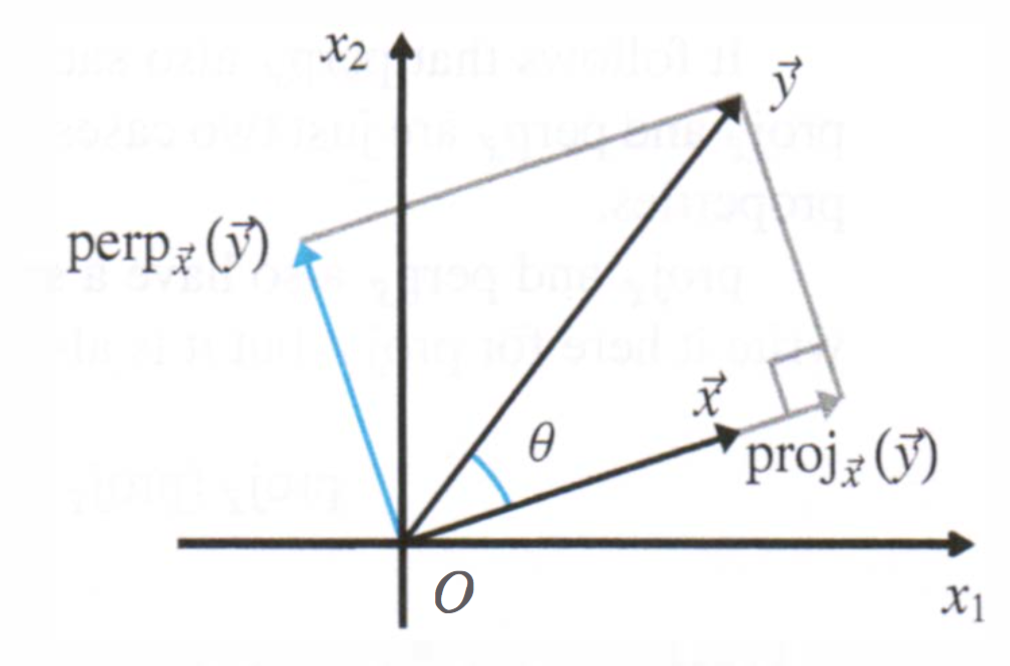
\includegraphics[scale=0.3]{perp_proj} \par}

\begin{enumerate}[label=\bfseries (\arabic*)] \itemsep0pt \parskip0pt 
    \item $proj_{\vec{x}} (\vec{y} + \vec{z}) = proj_{\vec{x}} \vec{y} + proj_{\vec{x}} \vec{z} \>$ for all $\vec{y}, \vec{z} \in \mathbb{R}^n$
    \item $proj_{\vec{x}} (t \vec{y}) = t proj_{\vec{x}} \vec{y} \>$ for all $\vec{y} \in \mathbb{R}^n$ and all $t \in \mathbb{R}$
\end{enumerate}

% ================================================== %

\subsection{Cross product [1.5]}
The cross-product is a construction that is defined only in $\mathbb{R}^3$. There is a generalization to higher dimensions, but it is considerably more complicated.
\begin{equation} \label{1.5-1}
    \begin{split}
        \vec{u} \times \vec{v} & = \begin{bmatrix}u_2 v_3 - u_3 v_2 \\ u_3 v_1 - u_1 v_3 \\ u_1 v_2 - u_2 v_1 \end{bmatrix}
    \end{split}
\end{equation}

\begin{enumerate}[label=\bfseries (\arabic*)] \itemsep0pt \parskip0pt 
    \item $\vec{x} \times \vec{y} = -\vec{y} \times \vec{x}$
    \item $\vec{x} \times \vec{x} = \vec{0}$
    \item $\vec{x} \times (\vec{y} + \vec{z}) = \vec{x} \times \vec{y} + \vec{x} \times \vec{z}$
    \item $(t \vec{x}) \times \vec{y} = t(\vec{x} \times \vec{y})$
\end{enumerate}

% ================================================== %

\subsection{Length of the cross product [1.5]}
Let $\vec{u}, \vec{v} \in \mathbb{R}^3$ and $\theta$ be the angle between $\vec{u}$ and $\vec{v}$, then
\begin{equation} \label{1.5-2}
    \begin{split}
        \|\vec{u} \times \vec{v}\| = \|\vec{u}\| \|\vec{v}\| \sin{\theta}
    \end{split}
\end{equation}
Which is the area of the parallelogram:

{\centering 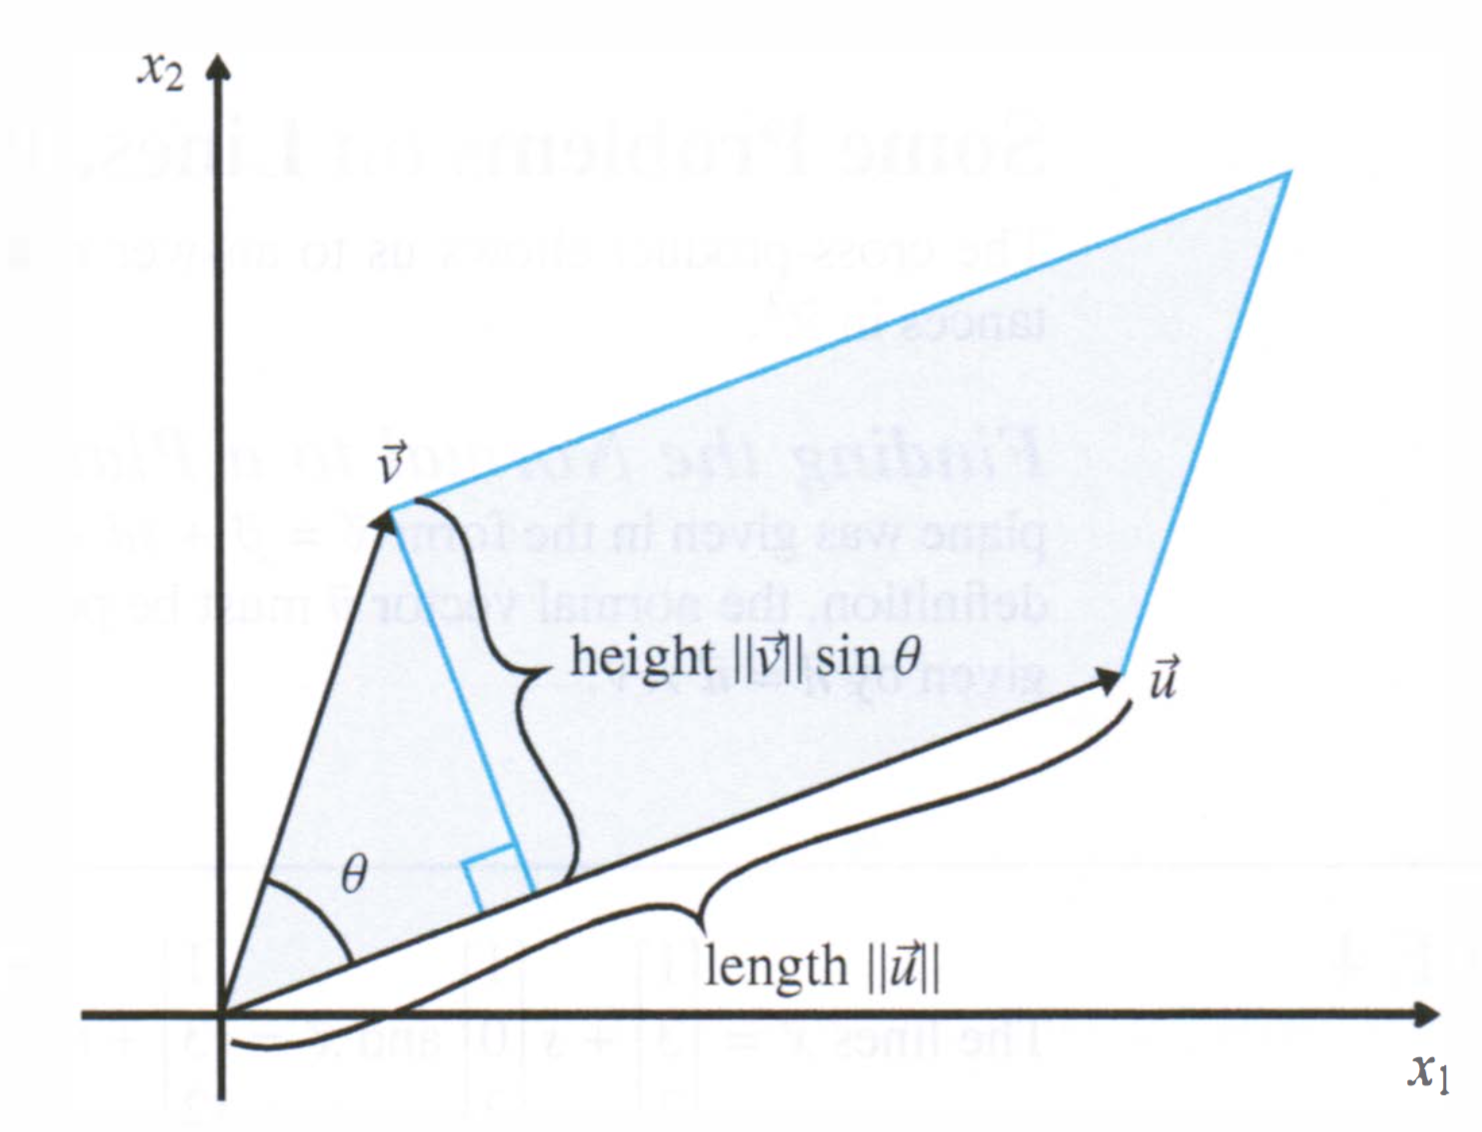
\includegraphics[scale=0.25]{area_cross} \par}



% ================================================== %
% == Systems of Linear Equations  == %
% ================================================== %

\section{Systems of Linear Equations}
A general system of $m$ linear equations in $n$ variables is written in the form
\begin{equation} \label{2.1-1}
    \begin{split}
        \vdots & \\
        a_{i1} + a_{i2} + \cdots + a_{ij} + \cdots + a_{in} & = b_i \\
        \vdots &
    \end{split}
\end{equation}

In matrix form:
\begin{equation} \label{2.1-2}
    \left[
    \begin{array}{cccccc|c}
        a_{11} & a_{12} & \cdots & a_{1j} & \cdots & a_{1n} & b_1 \\ 
        a_{21} & a_{22} & \cdots & a_{2j} & \cdots & a_{2n} & b_2 \\
        \vdots & \vdots & \ & \vdots & \ & \vdots & \vdots \\
        a_{i1} & a_{i2} & \cdots & a_{ij} & \cdots & a_{in} & b_i \\
        \vdots & \vdots & \ & \vdots & \ & \vdots & \vdots \\
        a_{m1} & a_{m2} & \cdots & a_{mj} & \cdots & a_{mn} & b_m
    \end{array}
    \right]
\end{equation}

% ================================================== %

\subsection{Elimination [2.1]}
Types of Steps in Elimination:
\begin{enumerate}[label=\bfseries (\arabic*)] \itemsep0pt \parskip0pt 
    \item Multiply one equation by a non-zero constant.
    \item Interchange two equations.
    \item Add a multiple of one equation to another equation.
\end{enumerate}

% ================================================== %

\subsection{Row Echelon Form [2.1]}
A matrix is in row echelon form \textbf{(REF)} if:
\begin{enumerate}[label=\bfseries (\arabic*)] \itemsep0pt \parskip0pt 
    \item When all entries in a row are zeros, this row appears below all rows that contain
a non-zero entry.
    \item When two non-zero rows are compared, the first non-zero entry, called the leading entry, in the upper row is to the left of the leading entry in the lower row.
\end{enumerate}

Any matrix can be row reduced to row echelon form by using the following steps:
\begin{enumerate}[label=\bfseries (\arabic*)] \itemsep0pt \parskip0pt 
    \item Consider the first column of the matrix; if it consists entirely of zero entries, move to the next column. If it contains some non-zero entry, interchange rows (if necessary) so that the top entry in the column is non-zero. We will call this entry a pivot.
    \item Use elementary row operations of type (3) to make all entries beneath the pivot into zeros.
    \item Next, consider the submatrix consisting of all columns to the right of the column we have just worked on and all rows below the row with the most recently obtained leading entry. Repeat the procedure described for this submatrix.
\end{enumerate}


% ================================================== %

\subsection{Consistent Systems and Unique Solutions [2.1]}
A system that has at least one solution is called \textbf{consistent}, and a system that does not have any solutions is called \textbf{inconsistent}.

Suppose that the augmented matrix $[A | \vec{b}]$ of a system of linear equations is row equivalent to $[S | \vec{c}]$, which is in row echelon form.

\begin{enumerate}[label=\bfseries (\arabic*)] \itemsep0pt \parskip0pt 
    \item The given system is inconsistent if and only if some row of $[S | \vec{c}]$ is of the form $[0 \> 0 \> \cdots \> 0 \> | \> c]$, with $c \neq 0$.
    \item If the system is consistent, there are two possibilities. Either the number of pivots in $S$ is equal to the number of variables in the system and the system has a unique solution, or the number of pivots is less than the number of variables and the system has infinitely many solutions.
\end{enumerate}

% ================================================== %

\subsection{Reduced Row Echelon Form [2.2]}
A matrix $R$ is said to be in \textbf{reduced row echelon form (RREF)} if
\begin{enumerate}[label=\bfseries (\arabic*)] \itemsep0pt \parskip0pt 
    \item It is in row echelon form.
    \item All leading entries are 1, called a \textbf{leading 1}.
    \item In a column with a leading 1, all the other entries are zeros.
\end{enumerate}
For any given matrix $A$ there is a unique matrix in reduced row echelon form that is row equivalent to $A$.

% ================================================== %

\subsection{Rank of a Matrix [2.2]}
The rank of a matrix $A$ is the number of leading 1s in its reduced row echelon form and is denoted by $rank(A)$.

Let $[A | \vec{b}]$ be a system of $m$ linear equations in $n$ variables.
\begin{enumerate}[label=\bfseries (\arabic*)] \itemsep0pt \parskip0pt 
    \item The system is consistent if and only if the rank of the coefficient matrix $A$ is
equal to the rank of the augmented matrix $[A | \vec{b}]$.
    \item If the system is consistent, then the number of parameters in the general solution is the number of variables minus the rank of the matrix: \#of parameters $= n - rank(A)$
\end{enumerate}

Let $[A | \vec{b}]$ be a system of $m$ linear equations in $n$ variables. Then $[A | \vec{b}]$ is consistent for all $\vec{b}$ if and only if $rank(A) = m$.

% ================================================== %

\subsection{Homogeneous Linear Equations [2.2]}
A linear equation is \textbf{homogeneous} if the right-hand side is zero. A system of linear equations is \textbf{homogeneous} if all of the equations of the system are homogeneous.

Observe that every homogeneous system is consistent as the zero vector $\vec{0}$ (the trivial solution) will certainly be a solution.

% ================================================== %

\subsection{Spanning Problems [2.3]}
A set of $k$ vectors $\{\vec{v_1}, ... ,\vec{v_k}\}$ in $\mathbb{R}^n$ spans $\mathbb{R}^n$ if and only if the rank of the coefficient matrix of the system $t_1 \vec{v_1} + ... + t_k \vec{v_k} = \vec{v}$ is $n$.

Let $\{\vec{v_1}, ... ,\vec{v_k}\}$ be a set of $k$ vectors in $\mathbb{R}^n$. If $Span\{\vec{v_1}, ... ,\vec{v_k}\} = \mathbb{R}^n$, then $k \leq n$.

% ================================================== %

\subsection{Linear Independence Problems [2.3]}
A set of $k$ vectors $\{\vec{v_1}, ... ,\vec{v_k}\}$ in $\mathbb{R}^n$ is linearly independent if and only if the rank of the coefficient matrix of the system $t_1 \vec{v_1} + ... + t_k \vec{v_k} = \vec{0}$ is $k$.

If $\{\vec{v_1}, ... ,\vec{v_k}\}$ is a linearly independent set of vectors in $\mathbb{R}^n$, then $k \leq n$.

% ================================================== %

\subsection{Bases of Subspaces [2.3]}
A set of $k$ vectors $\{\vec{v_1}, ... ,\vec{v_n}\}$ is a basis for $\mathbb{R}^n$ if and only if the rank of the coefficient matrix of $t_1 \vec{v_1} + ... + t_n \vec{v_n} = \vec{v}$ is $n$.

Suppose that $S$ is a non-trivial subspace of $\mathbb{R}^n$ and $Span\{\vec{v_1}, ... ,\vec{v_l}\} = S$. If $\{\vec{u_1}, ... ,\vec{u_k}\}$ is a linearly independent set of vectors in $S$, then $k \leq l$.

If $\{\vec{v_1}, ... ,\vec{v_l}\}$ and $\{\vec{u_1}, ... ,\vec{v_k}\}$ are both bases of a non-trivial subspace $S$ of $\mathbb{R}^n$, then $k = l$.

If S is a non-trivial subspace of $\mathbb{R}^n$ with a basis containing $k$ vectors, then we say that the \textbf{dimension} of $S$ is $k$ and write:
$$dim(S) = k$$

% ================================================== %


% ================================================== %
% == Matrices, Linear Mappings, and Inverses  == %
% ================================================== %

\section{Matrices, Linear Mappings, and Inverses}
We denote the $ij$-th entry of a matrix $A$ by $(A)_{ij}$.

% ================================================== %

\subsection{Triangular Matrix [3.1]}
A \textbf{square matrix} $U$ is \textbf{upper triangular} if the entries beneath the main diagonal are all zero. The \textbf{square matrix} $L$ is \textbf{lower triangular} if the entries above the main diagonal are all zero.

A matrix $D$ that is \textbf{both upper and lower triangular} is called a \textbf{diagonal matrix}. We denote an $n \times n$ diagonal matrix by $D = diag(d_{11}, d_{22}, \cdots, d_{nn})$.

% ================================================== %

\subsection{Addition and Scalar Multiplication [3.1]}
\begin{equation} \label{3.1-1}
    \begin{split}
        (A + B)_{ij} & = A_{ij} + B_{ij} \\
        (t A_{ij}) & = t (A_{ij})
    \end{split}
\end{equation}

\noindent Let $A, B, C$ be $m \times n$ matrices and let $s, t \in \mathbb{R}$. Then
\begin{enumerate}[label=\bfseries (\arabic*)] \itemsep0pt \parskip0pt 
    \item $A + B$ is an $m \times n$ matrix \textbf{(closed under addition)}
    \item $A + B = B + A$ \textbf{(addition is commutative)}
    \item $(A + B) + C = A + (B + C)$ \textbf{(addition is associative)}
    \item $\exists \ O{m,n}: A + O{m,n} = A$; It is the $m \times n$ matrix with all entries as zero, called the zero matrix \textbf{(zero vector)}
    \item $\forall A: \exists -(A), A + (-A) = O{m,n}$ \textbf{(additive inverse)}
    \item $sA$ is an $m \times n$ matrix \textbf{(closed under scalar multiplication)}
    \item $s(t A) = (st) A$ \textbf{(scalar multiplication is associative)}
    \item $(s + t) A = s A + t A$ \textbf{(distributive la)}
    \item $s(A + B) = s A + s B$ \textbf{(distributive law )}
    \item $1 A = A$ \textbf{(scalar multiplicative identity)}
\end{enumerate}

% ================================================== %

\subsection{Span and linear dependence [3.1]}
Let $\mathcal{B} = \{A_1, \cdots, A_k\}$ be a set of $m \times n$ matrices. Then the span of $\mathcal{B}$ is defined as:
\begin{equation} \label{3.1-2}
    \begin{split}
        Span \mathcal{B} = \{t_1 A_1, \cdots, t_k A_k \ | \ t_1, \cdots, t_k \in \mathbb{R} \}
    \end{split}
\end{equation}

$\mathcal{B}$ is \textbf{linearly independent} if the only solution to the equation $t_1 A_1 + \cdots + t_k A_k = O_{mn}$ is $t_1 = \cdots = t_k = 0$; otherwise $\mathcal{B}$ is \textbf{linearly dependent}.

% ================================================== %

\subsection{Transpose [3.1]}
\begin{equation} \label{3.1-3}
    \begin{split}
        (A^T)_{ij} = (A)_{ji}
    \end{split}
\end{equation}

For any matrices $A$ and $B$ and scalar $s \in \mathbb{R}$, we have
\begin{enumerate}[label=\bfseries (\arabic*)] \itemsep0pt \parskip0pt 
    \item $(A^T)^T = A$
    \item $(A + B)^T = A^T + B^T$
    \item $(s A)^T = s A^T$
\end{enumerate}

% ================================================== %

\subsection{Matrix Multiplication [3.1]}
\begin{equation} \label{3.1-4}
    \begin{split}
        A \vec{x} & = \begin{bmatrix}a_{11} & a_{12} \\ a_{21} & a_{22}\end{bmatrix} \begin{bmatrix}x_1 \\ x_2\end{bmatrix} = \begin{bmatrix}a_{11} x_1 & a_{12} x_2 \\ a_{21} x_1 & a_{22} x_2\end{bmatrix}
    \end{split}
\end{equation}

The matrix multiplication $BA$ of a $m \times n$ matrix $B$ and $n \times p$ matrix $A$ returns the $m \times p$ matrix whose $ij$-th entry is
\begin{equation} \label{3.1-5}
    \begin{split}
        (BA)_{ij} & = \vec{b_i} \cdot \vec{a_j}
    \end{split}
\end{equation}

If $A, B,$ and $C$ are matrices of the correct size so that the required products are defined, and $t \in \mathbb{R}$, then
\begin{enumerate}[label=\bfseries (\arabic*)] \itemsep0pt \parskip0pt 
    \item $A(B + C) = AB + AC$
    \item $(A + B)C = AC + BC$
    \item $t(AB) = (tA)B = A(tB)$
    \item $A(BC) = (AB)C$
    \item $(AB)^T = B^TA^T$
\end{enumerate}

There is \textbf{no division for matrices} because of the missing cancellation law for matrix multiplication.

The \textbf{identity matrix} with any $m \times n$ matrix:
\begin{equation} \label{3.1-6}
    \begin{split}
        I_m A = A = A I_n \ ; \ I_n & = \begin{bmatrix} \vec{e_1} & \cdots & \vec{e_n}\end{bmatrix} = \begin{bmatrix}1 & 0 & 0 \\ 0 & \ddots & 0 \\ 0 & 0 & 1 \end{bmatrix}
    \end{split}
\end{equation}

% ================================================== %

\subsection{Matrix Mappings [3.2]}
For any $m \times n$  matrix $A$, we define a function $f_A: \mathbb{R}^n \to \mathbb{R}^m$ called the \textbf{matrix mapping}, corresponding to $A$ by
\begin{equation} \label{3.2-1}
    \begin{split}
        f_A(\vec{x}): A \vec{x}
    \end{split}
\end{equation}
for any $\vec{x} \in \mathbb{R}^n$.

Then, for any $\vec{x}, \vec{y} \in \mathbb{R}^n$ and any $t \in \mathbb{R}$
\begin{enumerate}[label=\bfseries (L\arabic*)] \itemsep0pt \parskip0pt 
    \item $f_A(\vec{x} + \vec{y}) = f_A(\vec{x}) + f_A(\vec{y})$
    \item $f_A(t \vec{x}) = t f_A(\vec{x})$
\end{enumerate}

% ================================================== %

\subsection{Linear Mappings [3.2]}
A function $L: \mathbb{R}^n \to \mathbb{R}^m$ is called a \textbf{linear mapping (or linear transformation)} if for every $\vec{x}, \vec{y} \in \mathbb{R}^n$ and any $t \in \mathbb{R}$ it satisfies the following properties:
\begin{enumerate}[label=\bfseries (L\arabic*)] \itemsep0pt \parskip0pt 
    \item $L(\vec{x} + \vec{y}) = L(\vec{x}) + L(\vec{y})$
    \item $L(t \vec{x}) = t L(\vec{x})$
\end{enumerate}

A \textbf{linear operator $L$ on $\mathbb{R}^n$} is a linear mapping whose domain and codomain are the same.

If $L: \mathbb{R}^n \to \mathbb{R}^m$ is a linear mapping, then $L$ can be represented as a matrix mapping, with corresponding $m \times n$ matrix $[L]$ given by
\begin{equation} \label{3.2-2}
    \begin{split}
        [L] = \begin{bmatrix}L(\vec{e_1}) & L(\vec{e_2}) & \cdots & L(\vec{e_n}) \end{bmatrix}
    \end{split}
\end{equation}

% ================================================== %

\subsection{Compositions and Linear Combinations
of Linear Mappings [3.2]}
If L and M are linear mappings from $\mathbb{R}^n \to \mathbb{R}^m$ and $t \in \mathbb{R}$,then $(L + M)$ and $(t L)$ are linear mappings.

Let $L: \mathbb{R}^n \to \mathbb{R}^m$ and $M: \mathbb{R}^m \to \mathbb{R}^p$ be linear mappings. The \textbf{composition} $M \circ L: \mathbb{R}^n \to \mathbb{R}^p$ is defined by 
\begin{equation} \label{3.2-3}
    \begin{split}
        (M \circ L)(\vec{x}) = M(L(\vec{x}))
    \end{split}
\end{equation}
for all $\vec{x} \in \mathbb{R}^n$.

\noindent \\ Since compositions and linear combinations of linear mappings are linear mappings, it is natural to ask about the standard matrix of these new linear mappings.

Let $L: \mathbb{R}^n \to \mathbb{R}^m$, $M: \mathbb{R}^n \to \mathbb{R}^m$ and $N: \mathbb{R}^m \to \mathbb{R}^p$ be linear mappings and $t \in \mathbb{R}$. Then
\begin{equation} \label{3.2-4}
    \begin{split}
        [L + M] = [L] + [M], \> [t L] = t[L], \> [N \circ L] = [N][L]
    \end{split}
\end{equation}

% ================================================== %

\subsection{Identity Mapping [3.2]}
The linear mapping a $Id: \mathbb{R}^n \to \mathbb{R}^n$ defined by
\begin{equation} \label{3.2-5}
    \begin{split}
        Id(\vec{x}) = \vec{x}
    \end{split}
\end{equation}
is called the \textbf{identity mapping}.

% ================================================== %

\subsection{Geometrical Transformations [3.3]}

\subsubsection{Rotations in the plane}
$R_{\theta} : \mathbb{R}^2 \to \mathbb{R}^2$ is defined to be the transformation that rotates $\vec{x}$ counterclockwise through angle $\theta$ to the image $R_{\theta}(\vec{x})$.

\begin{equation} \label{3.3-1}
    \begin{split}
        R_{\theta}(\vec{x}) & = \begin{bmatrix}x_1 \cos{\theta} - x_2 \sin{\theta} \\ x_1 \sin{\theta} + x_2 \cos{\theta}\end{bmatrix}
    \end{split}
\end{equation}

{\centering 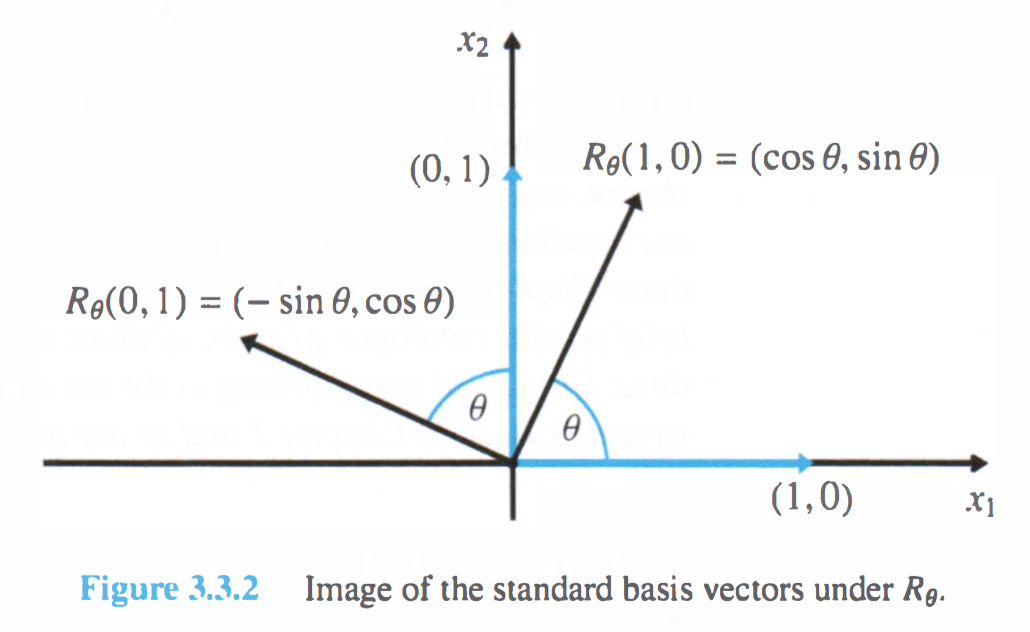
\includegraphics[scale=0.4]{rotation_plane} \par}

% -------------------------------------------------- %

\subsubsection{Rotation Through Angle $\theta$ about the $x_3$-axis in $\mathbb{R}^3$}
\begin{equation} \label{3.3-3}
    \begin{split}
        [R] & = \begin{bmatrix}\cos{\theta} && -\sin{\theta} && 0 \\ \sin{\theta} && \cos{\theta} && 0 \\ 0 && 0 && 1\end{bmatrix}
    \end{split}
\end{equation}

{\centering 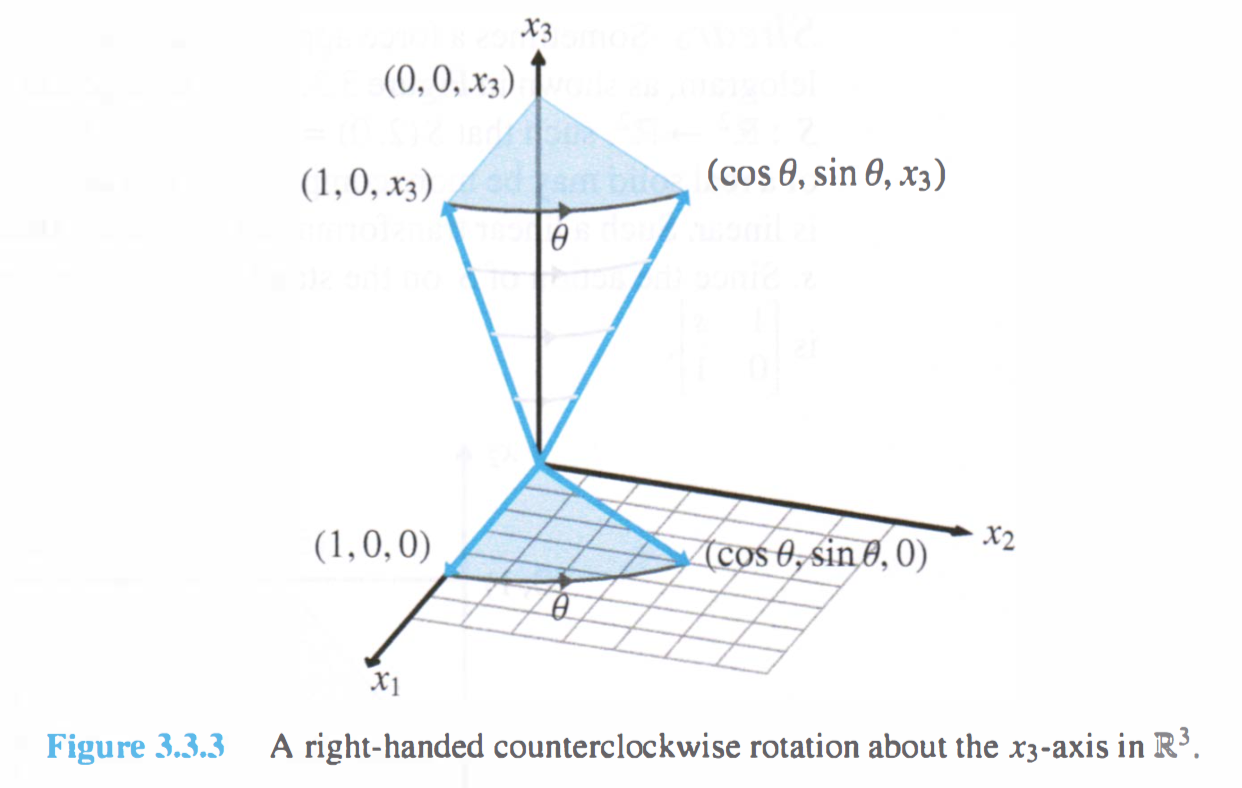
\includegraphics[scale=0.4]{rotation_about_z} \par}

% -------------------------------------------------- %

\subsubsection{Stretch/Shrink}
Example of a stretch (shrink for $t < 1$) in $x_1$-direction in $\mathbb{R}^2$:
\begin{equation} \label{3.3-4}
    \begin{split}
        [R] & = \begin{bmatrix}t && 0 \\ 0 && 1\end{bmatrix}
    \end{split}
\end{equation}

Stretching / shrinking in all directions is called \textbf{dilation} / \textbf{contraction}.

% -------------------------------------------------- %

\subsubsection{Shear}
\begin{equation} \label{3.3-5}
    \begin{split}
        [R] & = \begin{bmatrix}1 && s \\ 0 && 1\end{bmatrix}
    \end{split}
\end{equation}

{\centering 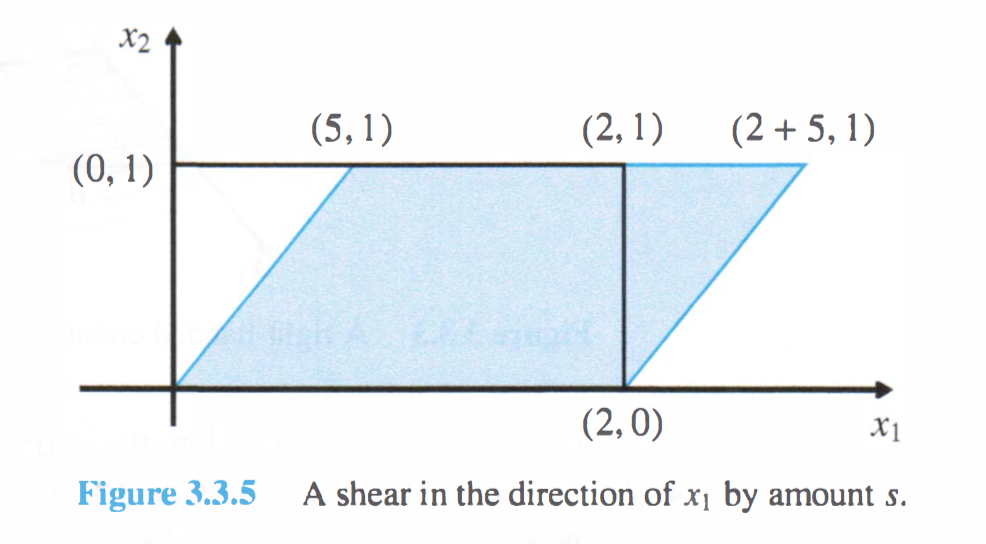
\includegraphics[scale=0.4]{shear} \par}

% -------------------------------------------------- %

\subsubsection{Reflections}
Examples: $a)$ reflection in $x_1$-axis, $b)$ reflection in the $x_1 x_2$-plane.
\begin{equation} \label{3.3-6}
    \begin{split}
        a) \> \begin{bmatrix}1 && 0 \\ 0 && -1\end{bmatrix}& \>\>\> b) \> \begin{bmatrix}1 && 0 && 0 \\ 0 && 1 && 0 \\ 0 && 0 && -1\end{bmatrix}
    \end{split}
\end{equation}

% -------------------------------------------------- %

\subsubsection{General reflections}
We consider only reflections in (or "across") lines in $\mathbb{R}^2$ or planes in $\mathbb{R}^3$ that pass through the origin. Reflections in lines or planes not containing the origin involve translations (which are not linear) as well as linear mappings.

Consider the plane in $\mathbb{R}^3$ with equation $\vec{n} \cdot \vec{x} = 0$. Since a reflection is related to $proj_{\vec{n}}$, a \textbf{reflection in the plane with normal vector $\vec{n}$} will be denoted \textbf{$refl_{\vec{n}}$}.

{\centering 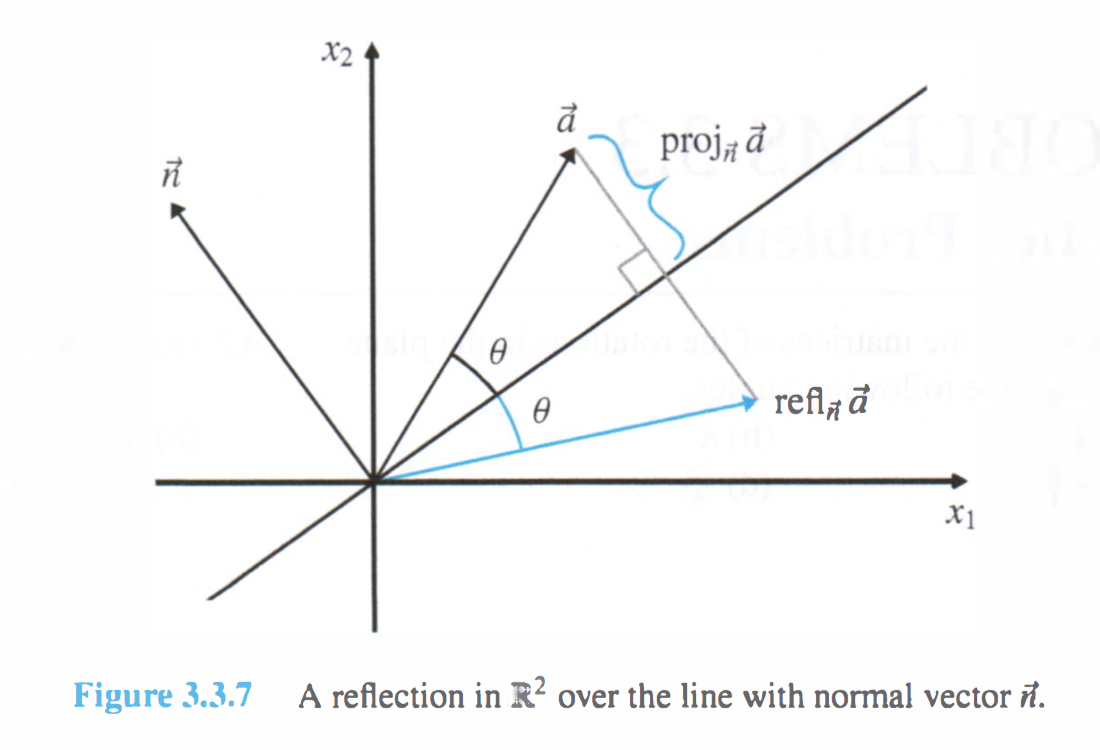
\includegraphics[scale=0.4]{general_reflection} \par}

% ================================================== %

\subsection{Solution Space [3.4]}
The set $S = \{\vec{x} \in \mathbb{R}^n | A \vec{x} = \vec{0}\}$ of all solutions to a homogeneous system $A \vec{x} = \vec{0}$ is called the \textbf{solution space} of the system $A \vec{x} = \vec{0}$.

% ================================================== %

\subsection{Null Space / Kernel [3.4]}
The \textbf{nullspace/kernel} of a linear mapping $L$ is the set of all vectors whose image under $L$ is the zero vector $\vec{0}$. This is also valid for matrices, where $A$ is an $m \times n$ matrix.

\begin{equation} \label{3.4-1}
    \begin{split}
        Null(L) & = ker(L) = \{\vec{x} \in \mathbb{R}^n | L(\vec{x}) = \vec{0}\} \\
        Null(A) & = ker(A) = \{\vec{x} \in \mathbb{R}^n | A \vec{x} = \vec{0}\}
    \end{split}
\end{equation}

% ================================================== %

\subsection{Solution Set of $A \vec{x} = \vec{b}$ [3.4]}
Let $\vec{p}$ be a solution of the system of linear equations $A \vec{x} = \vec{b}, \vec{b} \neq \vec{0}$.

\begin{enumerate}[label=\bfseries (\arabic*)] \itemsep0pt \parskip0pt 
    \item If $\vec{v}$ is any other solution of the same system, then $A(\vec{p} - \vec{v}) = \vec{0}$, so that $\vec{p} - \vec{v}$ is a solution of the corresponding homogeneous system $A \vec{x} = \vec{0}$.
    \item If $\vec{h}$ is any solution of the corresponding system $A \vec{x} = \vec{0}$, then $\vec{p} + \vec{h}$ is a solution of the system $A \vec{x} = \vec{b}$.
\end{enumerate}

% ================================================== %

\subsection{Range of $L$ and Columnspace of $A$ [3.4]}
\textbf{Range} of linear mapping $L: \mathbb{R}^n \to \mathbb{R}^m$ is defined to be the set
\begin{equation} \label{3.4-2}
    \begin{split}
        Range(L) & = \{L(\vec{v}) \in \mathbb{R}^m | \vec{x} \in \mathbb{R}^n\}
    \end{split}
\end{equation}

\noindent \textbf{Columnspace} of $m \times n$ matrix $A$ is the set $Col(A)$ defined by
\begin{equation} \label{3.4-3}
    \begin{split}
        Col(A) & = \{A \vec{v} \in \mathbb{R}^m | \vec{x} \in \mathbb{R}^n\}
    \end{split}
\end{equation}

The system of equations $A \vec{x} = \vec{b}$ is consistent if and only if $b$ is in the range of the linear mapping $L$ with standard matrix $A$ (or, equivalently, if and only if $b$ is in the columnspace of $A$).

% ================================================== %

\subsection{Rowspace of $A$ [3.4]}
Given an $m \times n$ matrix $A$, the \textbf{rowspace} of $A$ is the subspace spanned by the rows of $A$ (regarded as vectors) and is denoted $Row(A)$. Example:
\begin{equation} \label{3.4-4}
    \begin{split}
        Row(\begin{bmatrix}1 && 3 \\ 2 && -1 \\ 0 && 1\end{bmatrix}) & = Span\{ \begin{bmatrix}1 \\ 3\end{bmatrix}, \begin{bmatrix}2 \\ -1\end{bmatrix}, \begin{bmatrix}0 \\ 1\end{bmatrix}\}
    \end{split}
\end{equation}

% ================================================== %

\subsection{Bases for $Row(A)$, $Col(A)$, and $Null(A)$ [3.4]}
\textbf{Rowspace:} Let $B$ be the reduced row echelon form of an $m \times n$ matrix $A$.Then the non-zero rows of $B$ form a basis for $Row(A)$, and hence the dimension of $Row(A)$ equals the rank of $A$.\\

\textbf{Columnspace:} Suppose that $B$ is the reduced row echelon form of $A$. Then the columns of $A$ that correspond to the columns of $B$ with leading $1$s form a basis of the columnspace of $A$. Hence, the dimension of the columnspace equals the rank of $A$.\\

Let $A$ be an $m \times n$ matrix. We call the dimension of the nullspace of $A$ the \textbf{nullity} of $A$ and denote it by $nullity(A)$.

\textbf{Nullspace/Kernel:} Let $A$ be an $m \times n$ matrix with $rank(A) = r$. Then the spanning set for the general solution of the homogeneous system $A \vec{x} = \vec{0}$ is a basis for $Null(A)$ and the nullity of $A$ is $n - r$.

% ================================================== %

\subsection{Rank Theorem $A$ [3.4]}
If $A$ is any $m \times n$ matrix, then
\begin{equation} \label{3.4-5}
    \begin{split}
        rank(A) + nullity(A) & = n
    \end{split}
\end{equation}

Facts about Rank:
\begin{equation} \label{3.4-6}
    \begin{split}
        rank(A) & = \textrm{the number of leading 1s in the RREF of} A \\
        & = \textrm{the number of non-zero rows in any REF of} A \\
        & = dim Row(A) \\
        & = dim Col(A) \\
        & = n - dim Null(A)
    \end{split}
\end{equation}

% ================================================== %

\subsection{Inverse [3.5]}
Let $A$ be an $n \times n$ matrix. If there exists an $n \times n$ matrix $B$ such that $AB = I = BA$, then $A$ is said to be invertible, and $B$ is called the \textbf{inverse} of $A$ (and $A$ is the inverse of $B$). The inverse of $A$ is denoted $A^{-1}$. \\

\noindent Suppose that $A$ and $B$ are $n \times n$ matrices:
\begin{enumerate}[label=\bfseries (\arabic*)] \itemsep0pt \parskip0pt 
    \item $BA = AB = I$ and $CA = AC = I$. Then $B = C$.
    \item $AB = I$. Then $BA = I$, so that $B = A^{-1}$. Moreover, $B$ and $A$ have rank $n$.
\end{enumerate}

\noindent Suppose that $A$ and $B$ are invertible matrices and that $t$ is a non-zero real number:
\begin{enumerate}[label=\bfseries (\arabic*)] \itemsep0pt \parskip0pt 
    \item $(tA)^{-1} = \frac{1}{t} A^{-1}$
    \item $(AB)^{-1} = B^{-1} A^{-1}$
    \item $(A^T)^{-1} = (A^{-1})^T$
\end{enumerate}

% ================================================== %

\subsection{Finding $A^{-1}$[3.5]}
To find the inverse of a square matrix $A$,
\begin{enumerate}[label=\bfseries (\arabic*)] \itemsep0pt \parskip0pt 
    \item Row reduce the multi-augmented matrix $[ \> A \> | \> I \> ]$ so that the left block is in RREF.
    \item If the RREF is $[ \> I \> | \> B \> ]$ then $A^{-1} = B$.
    \item Else $A$ is not invertible.
\end{enumerate}

% ================================================== %

\subsection{Invertible Matrix Theorem [3.5]}
Suppose that $A$ is an $n \times n$ matrix. Then the following statements are equivalent (that is, one is true if and only if each of the others is true).

\begin{enumerate}[label=\bfseries (\arabic*)] \itemsep0pt \parskip0pt 
    \item $A$ is invertible.
    \item $rank(A) = n$
    \item The reduced row echelon form of $A$ is $I$.
    \item For all $b \in \mathbb{R}^n$, the system $A \vec{x} = \vec{b}$ is consistent and has a unique solution.
    \item The columns of $A$ are linearly independent.
    \item The columnspace of $A$ is $\mathbb{R}^n$.
\end{enumerate}

Suppose that $L: \mathbb{R}^n \to \mathbb{R}^n$ is a linear mapping with standard matrix $A = [l]$. Then, the following statements are equivalent to each other and to the statements above.

\begin{enumerate}[label=\bfseries (\arabic*)] \itemsep0pt \parskip0pt 
    \setcounter{enumi}{6}
    \item $L$ is invertible.
    \item $range(L) = \mathbb{R}^n$
    \item $Null(L) = \{\vec{0}\}$
\end{enumerate}

% ================================================== %

% \subsection{Elementary Matrices [3.6]}
% Not part of this course.

% \subsection{LU-Decomposition [3.7]}
% Not part of this course.



% ================================================== %
% == Vector Spaces  == %
% ================================================== %

\section{Vector Spaces}

\subsection{Spaces of polynomials [4.1]}

\subsubsection{Addition and Scalar Multiplication of Polynomials}

Let $p(x)$, $q(x)$ and $r(x)$ be polynomials of degree at most $n$ and let $s, t \in \mathbb{R}$. Then:
\begin{enumerate}[label=\bfseries (\arabic*)] \itemsep0pt \parskip0pt 
    \item $p(x) + q(x)$ is a polynomial of degree at most $n$
    \item $p(x) + q(x) = q(x) + p(x)$
    \item $(p(x) + q(x)) + r(x) = p(x) + (q(x) + r(x))$
    \item The polynomial $0 = 0 + 0x + \cdots + 0x^n$, called the \textbf{zero polynomial}, satisfies $p(x) + 0 = p(x) = 0 + p(x)$ for any polynomial $p(x)$
    \item For each polynomial $p(x)$, there exists an additive inverse, denoted $(-p)(x)$, with the property that $p(x) + (-p)(x) = 0$; in particular, $(-p)(x) = -p(x)$
    \item $t p(x)$ is a polynomial of degree at most $n$
    \item $s(tp(x)) = (st)p(x)$
    \item $(s + t)p(x) = s p(x) + t p(x)$
    \item $t(p(x) + q(x)) = t p(x) + t q(x)$
    \item $1 p(x) = p(x)$
\end{enumerate}

% -------------------------------------------------- %

\subsubsection{Span}
Let $\mathcal{B} = \{p_1(x), ..., p_k(x)\}$ be a set of polynomials of degree at most $n$. Then the \textbf{span} of $\mathcal{B}$ is defined as 
\begin{equation} \label{4.1-1}
    \begin{split}
        Span \mathcal{B} & = \{t_1 p_1(x) + \cdots + t_k p_k(x) | t_1, ..., t_k \in \mathbb{R}\}
    \end{split}
\end{equation}

% -------------------------------------------------- %

\subsubsection{Linear Independent}
The set $\mathcal{B} = \{p_1(x), ..., p_k(x)\}$ is said to \textbf{linearly independent} if the only solution to the equation 
\begin{equation} \label{4.1-2}
    \begin{split}
        t_1 p_1(x) + \cdots + t_k p_k(x) = 0
    \end{split}
\end{equation}

is $t_1 = \cdots = t_k = 0$; otherwise, $\mathcal{B}$ is \textbf{linearly dependent}.

% ================================================== %

\subsection{Vector Spaces [4.2]}
A \textbf{vector space over $\mathbb{R}$} is a set $\mathbb{V}$ together with an operation of \textbf{addition} ($\oplus$), usually denoted $x + y$ for any $x, y \in \mathbb{V}$, and an operation of \textbf{scalar multiplication} ($\odot$), usually denoted $s x$ for any $x \in \mathbb{V}$ and $s \in \mathbb{R}$, such that for any $x, y, z \in \mathbb{V}$ and $s, t \in \mathbb{R}$ we have all of the following properties:

\begin{enumerate}[label=\bfseries V(\arabic*)] \itemsep0pt \parskip0pt 
    \item $x + y \in \mathbb{V}$ \textbf{(closed under addition)}
    \item $x + y = y + x$ \textbf{(addition is commutative)}
    \item $(x + y) + z = x + (y + z)$ \textbf{(addition is associative)}
    \item $\exists \> \textbf{0} \in \mathbb{V}: x + 0 = x = 0 + x$ \textbf{(zero vector)}
    \item $\forall x \in \mathbb{V}: \exists -x \in \mathbb{V}, x + (-x) = 0$ \textbf{(additive inverse)}
    \item $t x \in \mathbb{V}$ \textbf{(closed under scalar multiplication)}
    \item $s(t x) = (st)x$ \textbf{(scalar multiplication is associative)}
    \item $(s + t)x = s x + t x$ \textbf{(distributive la)}
    \item $t(x + y) = t x + t y$ \textbf{(distributive law )}
    \item $1 x = x$ \textbf{(scalar multiplicative identity)}
\end{enumerate}

Let $\mathbb{V}$ be a vector space. Then
\begin{enumerate}[label=\bfseries (\arabic*)] \itemsep0pt \parskip0pt 
    \item $0 x = 0 \forall x \in \mathbb{V}$
    \item $(-1) x = -x \forall x \in \mathbb{V}$
    \item $t 0 = 0 \forall t \in \mathbb{R}$
\end{enumerate}

% -------------------------------------------------- %

\subsubsection{Subspaces}
Suppose that $\mathbb{V}$ is a vector space. A non-empty subset $\mathbb{U}$ of $\mathbb{V}$ is a \textbf{subspace} $\mathbb{V}$ if it satisfies the following two properties:
\begin{enumerate}[label=\bfseries S(\arabic*)] \itemsep0pt \parskip0pt 
    \item $x + y \in \mathbb{U}, \> \forall x, y \in \mathbb{V}$ ($\mathbb{U}$ is closed under addition)
    \item $t x \in \mathbb{U}, \forall x \in \mathbb{U}$ and $t \in \mathbb{R}$ ($\mathbb{U}$ is closed under scalar multiplication)
\end{enumerate}

\textbf{Equivalent definition:} If $\mathbb{U}$ is a subset of a vector space $\mathbb{V}$ and $\mathbb{U}$ is also a vector space using the same operations as $\mathbb{V}$, then $\mathbb{U}$ is a \textbf{subspace} of $\mathbb{V}$.

% -------------------------------------------------- %

\subsubsection{Set of all possible linear combinations}
If $\{v_1(x), ..., v_k(x)\}$ is a set of vectors in a vector space $\mathbb{V}$ and $\mathbb{S}$ is the set of all possible linear combinations of these vectors,
\begin{equation} \label{4.2-1}
    \begin{split}
        \mathbb{S} = \{t_1 v_1 + \cdots + t_k v_k \> | t_1, ..., t_k \in \mathbb{R}\}
    \end{split}
\end{equation}

then $\mathbb{S}$ is a subspace of $\mathbb{V}$.

% -------------------------------------------------- %

\subsubsection{Span, Spanning Set}
If $\mathbb{S}$ is the subspace of the vector space $\mathbb{V}$ consisting of all possible linear combinations of the vectors $v_1, ..., v_k \in \mathbb{V}$, then $\mathbb{S}$ is called the subspace spanned by $\mathcal{B} = \{v_1, ..., v_k\}$, and we say that set $\mathcal{B}$ \textbf{spans} $\mathbb{S}$. The set $\mathcal{B}$ is called a \textbf{spanning set} for the subspace $\mathbb{S}$. We denote $\mathbb{S}$ by
\begin{equation} \label{4.2-2}
    \begin{split}
        \mathbb{S} & = Span \{t_1 p_1(x) + \cdots + t_k p_k(x)\} = Span \mathcal{B}
    \end{split}
\end{equation}

% -------------------------------------------------- %

\subsubsection{Linear Independence}
If $\mathcal{B} = \{p_1(x), ..., p_k(x)\}$ is a set of vectors in vector space $\mathbb{V}$, then $\mathcal{B}$ is said to \textbf{linearly independent} if the only solution to the equation 
\begin{equation} \label{4.2-3}
    \begin{split}
        t_1 p_1(x) + \cdots + t_k p_k(x) = 0
    \end{split}
\end{equation}

is $t_1 = \cdots = t_k = 0$; otherwise, $\mathcal{B}$ is \textbf{linearly dependent}.

% ================================================== %

\subsection{Bases [4.3]}

Let $\mathcal{B} = \{v_1, ..., v_n\}$ be a spanning set for a vector space $\mathbb{V}$. Then every vector in $\mathbb{V}$ can be expressed in a \textit{unique way} as a linear combination of the vectors of $\mathcal{B}$ if and only if the set $\mathcal{B}$ is linearly independent.

A set $\mathbb{B}$ of vectors in a vector space $\mathcal{V}$ is a \textbf{basis} if it is a linearly independent spanning set for $\mathbb{V}$.

% -------------------------------------------------- %

\subsubsection{Dimension}
If a vector space $\mathbb{V}$ has a basis of $n$ vectors, then the \textbf{dimension} of $\mathbb{V}$ is $n$.
\begin{equation} \label{4.3-1}
    \begin{split}
        dim(\mathbb{V}) = n
    \end{split}
\end{equation}

% -------------------------------------------------- %

\subsubsection{Coordinate Vector}
The \textbf{coordinate vector} of x with respect to the basis $\mathcal{B}$ is denoted by
\begin{equation} \label{4.3-2}
    \begin{split}
        [x]{_\mathcal{B}} = \begin{bmatrix}x_1 \\ x_2 \\ \vdots \\ x_n \end{bmatrix}
    \end{split}
\end{equation}

% -------------------------------------------------- %

\subsubsection{Change of Coordinates Matrix}
Let $\mathcal{B}$ and $\mathcal{C} = \{w_1, ..., w_n\}$ both be bases for a vector space $\mathbb{V}$. The matrix $P = \begin{bmatrix}[w_1]_{\mathcal{B}} & \cdots & [w_n]_{\mathcal{B}}\end{bmatrix}$ is called the \textbf{change of coordinates matrix} from $\mathcal{C}$-coordinates to $\mathcal{B}$-coordinates and satisfies 
\begin{equation} \label{4.3-3}
    \begin{split}
        [x]_{\mathcal{B}} = P [x]_{\mathcal{C}}
    \end{split}
\end{equation}

\noindent then $P$ is invertible and $P^{-1}$ is the change of coordinates matrix from $\mathcal{B}$-coordinates to $\mathcal{C}$-coordinates.

% ================================================== %

\subsection{Linear Mappings [4.5]}
If $\mathbb{V}$ and $\mathbb{W}$ are vector spaces over $\mathbb{R}$, a function $L : \mathbb{V} \to \mathbb{W}$ is a linear mapping if it satisfies the linearity properties
\begin{enumerate}[label=\bfseries L\arabic*] \itemsep0pt \parskip0pt 
    \item L(x + y) = L(x) = L(y)
    \item L(t x) = t L(x)
\end{enumerate}
for all $x, y \in \mathbb{V}$ and $t \in \mathbb{R}$. If $\mathbb{W} = \mathbb{V}$, then $L$ may be called a \textbf{linear operator}.

% -------------------------------------------------- %

\subsubsection{Range}
Let $\mathbb{V}$ and $\mathbb{W}$ be vector spaces over $\mathbb{R}$. The \textbf{range} of a linear mapping $L: \mathbb{V} \to \mathbb{W}$ is defined to be the set
\begin{equation} \label{4.5-1}
    \begin{split}
        Range(L) = \{L(x) \in \mathbb{W} \> | \> x \in \mathbb{V}\}
    \end{split}
\end{equation}

\noindent The \textbf{nullspace} of $L$ is the set of all vectors in $\mathbb{V}$ whose image under $L$ is the zero vector $0_{\mathbb{W}}$. We write
\begin{equation} \label{4.5-2}
    \begin{split}
        Null(L) = \{x \in \mathbb{V} \> | \> L(x) = 0_{\mathbb{W}}\}
    \end{split}
\end{equation}

Let $\mathbb{V}$ and $\mathbb{W}$ be vector spaces and let $L : \mathbb{V} \to \mathbb{W}$ be a linear mapping. Then
\begin{enumerate}[label=\bfseries (\arabic*)] \itemsep0pt \parskip0pt 
    \item $L(0_{\mathbb{V}}) = 0_{\mathbb{W}}$
    \item $Null(L)$ is a subspace of $\mathbb{V}$
    \item $Range(L)$ is a subspace of $\mathbb{W}$
\end{enumerate}

% -------------------------------------------------- %

\subsubsection{Rank}
Let $\mathbb{V}$ and $\mathbb{W}$ be vector spaces over $\mathbb{R}$. The \textbf{rank of a linear mapping} $L: \mathbb{V} \to \mathbb{W}$ is the dimension of the range of $L$:
\begin{equation} \label{4.5-3}
    \begin{split}
        rank(L) = dim(Range(L))
    \end{split}
\end{equation}

% -------------------------------------------------- %

\subsubsection{Nullity}
Let $\mathbb{V}$ and $\mathbb{W}$ be vector spaces over $\mathbb{R}$. The \textbf{nullity of a linear mapping} $L: \mathbb{V} \to \mathbb{W}$ is the dimension of the nullspace of $L$:
\begin{equation} \label{4.5-4}
    \begin{split}
        nullity(L) = dim(Null(L))
    \end{split}
\end{equation}

\noindent Morever, if $dim(\mathbb{V}) = n$, then $rank(L) + nullity(L) = n$.

% ================================================== %

\subsection{Matrix of a Linear Mapping [4.6]}

Suppose that $\mathcal{B} = \{\vec{v}_1, ..., \vec{v}_2\}$ is any basis for a vector space $\mathbb{V}$ and that $L : \mathbb{V} \to \mathbb{V}$ is a linear operator. Define the \textbf{matrix of the linear operator} $L$ with respect to the basis $\mathcal{B}$ to be the matrix
\begin{equation} \label{4.6-1}
    \begin{split}
        [L]_{\mathcal{B}} = \begin{bmatrix}[L(\vec{v}_1)]_{\mathcal{B}} & \cdots & [L(\vec{v}_n)]_{\mathcal{B}}\end{bmatrix}
    \end{split}
\end{equation}

\noindent Then for any $\vec{x} \in \mathbb{R}^n$,
\begin{equation} \label{4.6-2}
    \begin{split}
        [L(\vec{x})]_{\mathcal{B}} = [L]_{\mathcal{B}} [\vec{x}]_{\mathcal{B}}
    \end{split}
\end{equation}

% -------------------------------------------------- %

\subsubsection{Change of Coordinates and Linear Mappings}
Let $\mathcal{S}$ denote the standard basis for $\mathbb{R}^n$ and let $\mathcal{B}$ be any other basis for $\mathbb{R}^n$. Then we have for the change of coordinates matrix $P$:
\begin{equation} \label{4.6-3}
    \begin{split}
        [L]_{\mathbb{B}} = P^{-1} [L]_{\mathcal{S}} P
    \end{split}
\end{equation}

% ================================================== %

% \subsection{Isomorphism of Vector Spaces [4.7]}
% Not part of this course.



% ================================================== %
% == Vector Spaces  == %
% ================================================== %

\section{Determinants}

% ================================================== %

\subsection{Calculation of $3 \times 3$ matrices [5.1]}
{\centering 
\includegraphics[scale=0.3]{determinant} \par}

% ================================================== %

\subsection{Calculation of $n \times n$ matrices [5.1]}
Let $A$ be a $n \times n$ matrix. Let $A(i,j)$ denote the $(n - 1) \times (n - 1)$ submatrix obtained from $A$ by deleting the $i$-th row and $j$-th column. The \textbf{cofactor of an $n \times n$ matrix of $a_{ij}$} is defined to be
\begin{equation} \label{5.1-1}
    \begin{split}
        C_{ij} = (-1)^{(i + j)} det A(i, j)
    \end{split}
\end{equation}

The \textbf{determinant of a $n \times n$ matrix A} is defined by
\begin{equation} \label{5.1-2}
    \begin{split}
        det A = a_{11} C_{11} + a_{12} C_{12} + \cdots + a_{1n} C_{1n}
    \end{split}
\end{equation}

The determinant of $A$ may be obtained by \textbf{cofactor expansion} along any row or any column.

% ================================================== %

\subsection{Theorems [5.1]}
Suppose that $A$ is an $n \times n$ matrix, then
\begin{enumerate}[label=\bfseries (\arabic*)] \itemsep0pt \parskip0pt 
    \item If one row (or column) of $A$ contains only zeros: $det A = 0$.
    \item If $A$ is an upper- or lower-triangular matrix, then the determinant of $A$ is the product of the diagonal entries of $A$: $det A = a_{11} a_{22} \cdots a_{nn}$
    \item $det A = det A^T$
\end{enumerate}

% ================================================== %

\subsection{Elementary Row Operations [5.2]}
Suppose that $A$ is an $n \times n$ matrix, then
\begin{enumerate}[label=\bfseries (\arabic*)] \itemsep0pt \parskip0pt 
    \item Multiplying a row of $A$ by a scalar $t$ has the effect $t(det A)$
    \item Adding one row to another has no effect on the determinant
    \item Swapping rows negates the determinant: $(-1)(det A)$
\end{enumerate}

% ================================================== %

\subsection{Invertibility [5.2]}
If $A$ is an $n \times n$ matrix, then the following are equivalent:
\begin{enumerate}[label=\bfseries (\arabic*)] \itemsep0pt \parskip0pt 
    \item $det A \neq 0$
    \item $rank(A) = n$
    \item A is invertible
\end{enumerate}

% ================================================== %

\subsection{Determinant of a Product [5.2]}
If $A$ and $B$ are $n \times n$ matrices, then
\begin{equation} \label{5.2-1}
    \begin{split}
        det(AB) = (det A)(det B)
    \end{split}
\end{equation}

% ================================================== %

\subsection{Matrix Inverse by Cofactors [5.3]}

% -------------------------------------------------- %

\subsubsection{Cofactor Matrix}
Let $A$ be an $n \times n$ matrix. We define the \textbf{cofactor matrix} of $A$:
\begin{equation} \label{5.3-1}
    \begin{split}
        (cof A)_{ij} = C_{ij}
    \end{split}
\end{equation}

% -------------------------------------------------- %

\subsubsection{Carmer's Rule}
Consider the system of $n$ linear equations in $n$ variables, $A \vec{x} = \vec{b}$. If $det A \neq 0$ so that $A$ is invertible, then the solution may be written in the form:
\begin{equation} \label{5.3-2}
    \begin{split}
        \vec{x} & = A^{-1} \vec{b} = \frac{1}{det A} (cof A)^T \vec{b} \\
        \begin{bmatrix}x_1 \\ \vdots \\ x_i \\ \vdots \\ x_n \end{bmatrix} & = \frac{1}{det A} \begin{bmatrix}C_{11} & C_{21} & \cdots & C_{n1} \\ \vdots & \vdots & \vdots & \vdots \\ C_{1i} & C_{2i} & \cdots & C_{ni} \\ \vdots & \vdots & \ddots & \vdots \\ C_{1n} & C_{2n} & \cdots  &C_{nn} \end{bmatrix}
    \end{split}
\end{equation}

% ================================================== %

\subsection{Area, Volume and the Derminant [5.4]}
Interesting geometric interpretations of the determinant value:

\begin{enumerate}[label=\bfseries (\arabic*)] \itemsep0pt \parskip0pt 
    \item The area of the parallelogram induced by $\vec{u}$ and $\vec{v}$ is $Area(\vec{u}, \vec{v}) = |det \begin{bmatrix}u_1 & v_1 \\ u_2 & v_2 \end{bmatrix}|$
    \item Similar, in 3 dimensions, for the parallelepid: $Volume(\vec{u}, \vec{v}, \vec{w}) = |det \begin{bmatrix}\vec{u} & \vec{v} & \vec{w}\end{bmatrix}|$. This works in general for n-dimensional parallelotopes with n-volume.
    \item The absolute value of the determinant of the standard matrix $A$ of a linear transformation is the factor by which the area is changed under the linear transformation $L$.
\end{enumerate}



% ================================================== %
% == Eigenvectors and Diagonalization  == %
% ================================================== %

\section{Eigenvectors and Diagonalization}

Suppose that $L : \mathbb{R}^n \to \mathbb{R}^n$ is a linear transformation. A non-zero vector $\vec{v} \in \mathbb{R}^n$ such that $L(\vec{v}) = \lambda \vec{v}$ is called an \textbf{eigenvector} of $L$; the scalar $\lambda$ is called an \textbf{eigenvalue} of $L$. The pair $\lambda, \vec{v}$ is called an \textbf{eigenpair}.

This also holds for an $n \times n$ matrix $A$, such that $A \vec{v} = \lambda \vec{v}$, for a non-zero vector $\vec{v} \in \mathbb{R}^n$.

% ================================================== %

\subsection{Finding Eigenvalues and Eigenvectors [6.1]}
Suppose that $A$ is an $n \times n$ matrix. A real number $\lambda$ is an eigenvalue of $A$ if and only if $\lambda$ satisfies the equation
\begin{equation} \label{6.1-1}
    \begin{split}
        det(A - \lambda I) = 0
    \end{split}
\end{equation}

If $\lambda$ is an eigenvalue of $A$, then all non-trivial solutions of the homogeneous system
\begin{equation} \label{6.1-2}
    \begin{split}
        (A - \lambda I) \vec{v} = 0
    \end{split}
\end{equation}
are eigenvectors of $A$ that correspond to $\lambda$.

Suppose that $\lambda_1, ..., \lambda_k$ are distinct ($\lambda_i \neq \lambda_j$) eigenvalues of an $n \times n$ matrix $A$, with corresponding eigenvectors $\vec{v}_1, ..., \vec{v}_k$, respectively. Then $\{\vec{v}_1, ..., \vec{v}_k\}$ is linearly independent.

% ================================================== %

\subsubsection{Eigenspaces}
Let $\lambda$ be an eigenvalue of an $n \times n$ matrix $A$. Then the set containing the zero vector and all eigenvectors of $A$ corresponding to $\lambda$ is called the \textbf{eigenspace} of $\lambda$.

% ================================================== %

\subsubsection{Characteristic Polynomials}
Let $A$ be an $n \times n$ matrix $A$. Then $C(\lambda) = det(A - \lambda I)$ is called the \textbf{characteristic polynomial} of $A$.

% -------------------------------------------------- %

\subsubsection{Algebraic and Geometric Multiplicity}
Let $A$ be an $n \times n$ matrix with eigenvalue $\lambda$. The \textbf{algebraic multiplicity} of $\lambda$ is the number of times $\lambda$ is repeated as a root of the characteristic polynomial. The \textbf{geometric multiplicity} of $\lambda$ of $\lambda$ is the dimension of the eigenspace of $\lambda$.
\begin{equation} \label{6.1-3}
    \begin{split}
        1 & \leq \textrm{geometric multiplicity} \leq \textrm{algebraic multiplicity}
    \end{split}
\end{equation}

% ================================================== %

\subsection{Diagonalization [6.2]}
\begin{equation} \label{6.2-1}
    \begin{split}
        P^{-1} A P = D = diag(\lambda_1, ..., \lambda_n)
    \end{split}
\end{equation}
If there exists an invertible matrix $P$ and diagonal matrix $D$ such that $P^{-1} A P = D$, then $A$ is \textbf{diagonalizable or diagonable} and matrix $P$ \textbf{diagonalizes} $A$ to its \textbf{diagonal form} $D$. \\

An $n \times n$ matrix $A$ is diagonalizable if and only if every eigenvalue of matrix A has its geometric multiplicity equal to its algebraic multiplicity. Or in other words, when $A$ has $n$ distinct eigenvalues. \\

If $A$ and $B$ are $n \times n$ matrices such that $P^{-1} A P = B$ for some invertible matrix $P$, then $A$ and $B$ have

\begin{enumerate}[label=\bfseries (\arabic*)] \itemsep0pt \parskip0pt 
    \item The same determinant
    \item The same eigenvalues
    \item The same rank
    \item The same \textbf{trace}, where the trace of a matrix $A$ is defined by $tr(A) = \sum^{n}_{i=1} a_{ii}$
\end{enumerate}

and are called \textbf{similar}.

% ================================================== %
% == Orthonormal Bases  == %
% ================================================== %

\section{Orthonormal Bases}

% ================================================== %

\subsection{Orthogonality [7.1]}
A set of vectors $\{\vec{v}_1, ..., \vec{v}_k\}$ in $\mathbb{R}^n$ is \textbf{orthogonal} if $\vec{v}_i \cdot \vec{v}_j = 0$ whenever $i \neq j$.

If $\{\vec{v}_1, ..., \vec{v}_k\}$ is an orthogonal set of non-zero vectors in $\mathbb{R}^n$, it is linearly independent.

% -------------------------------------------------- %

\subsubsection{Orthonormal}
A set of vectors $\{\vec{v}_1, ..., \vec{v}_k\}$ in $\mathbb{R}^n$ is \textbf{orthonormal} if it is orthogonal and each vector $\vec{v}_i$ is a unit vector (that is, each vector is normalized).

% -------------------------------------------------- %

\subsubsection{Coordinates with Respect to an ON-Basis}
If $\mathcal{B} = \{\vec{v}_1, ..., \vec{v}_n\}$ is an orthonormal basis for $\mathbb{R}^n$, then the $i$-th coordinate of a vector $\vec{x} \in \mathbb{R}^n$ with respect to $\mathcal{B}$ is
\begin{equation} \label{7.1-1}
    \begin{split}
        b_i = \vec{x} \cdot \vec{v}_i
    \end{split}
\end{equation}

Because the dot product of all other elements will be 0 (orthogonality). It follows that $\vec{x}$ can be written as
\begin{equation} \label{7.1-2}
    \begin{split}
        \vec{x} = (\vec{x} \cdot \vec{v}_1) \vec{v}_1 + (\vec{x} \cdot \vec{v}_2) \vec{v}_2 + \cdots + (\vec{x} \cdot \vec{v}_n) \vec{v}_n 
    \end{split}
\end{equation}

% -------------------------------------------------- %

\subsubsection{Change of Coordinates and Orthogonal Matrices}
An $n \times n$ matrix $P$ such that $P^T P = I$ is called an \textbf{orthogonal matrix}. It follows that $P^{-1} = P^T$ and that $P P^T = I = P^T P$.

The following are equivalent for an $n \times n$ matrix $P$:
\begin{enumerate}[label=\bfseries (\arabic*)] \itemsep0pt \parskip0pt 
    \item $P$ is an orthogonal matrix
    \item The columns of $P$ from an orthonormal set
    \item The rows of $P$ form an orthonormal set
\end{enumerate}

% ================================================== %

\subsection{Projections and Gram-Schmidt [7.2]}

% -------------------------------------------------- %

\subsubsection{Orthogonal Component}
Let $\mathbb{S}$ be a subspace of $\mathbb{R}^n$. We shall say that a vector $\vec{x}$ is \textbf{orthogonal} to $\mathbb{S}$ if $\vec{x} \cdot \vec{s} = 0, \forall \vec{s} \in \mathbb{S}$. We call the set of all vectors orthogonal to $\mathbb{S}$ the \textbf{orthogonal complement} of $\mathbb{S}$ and denote it $\mathbb{S}^\bot$. That is,
\begin{equation} \label{7.2-1}
    \begin{split}
        \mathbb{S}^\bot = \{\vec{x} \in \mathbb{R}^n \> | \> \vec{x} \cdot \vec{s} = 0, \forall \vec{s} \in \mathbb{S}\}
    \end{split}
\end{equation}

Let $\mathbb{S}$ be a $k$-dimensional subspace of $\mathbb{R}^n$. Then $\mathbb{S}$ is a subspace of $\mathbb{R}^n$ and:
\begin{enumerate}[label=\bfseries (\arabic*)] \itemsep0pt \parskip0pt 
    \item $\mathbb{S} \cap \mathbb{S}^\bot = \{\vec{0}\}$
    \item $dim(\mathbb{S}^\bot) = n - k$
    \item If $\{\vec{v}_1, ..., \vec{v}_k\}$ is an on-basis for $\mathbb{S}$ and $\{\vec{v}_{k + 1}, ..., \vec{v}_n\}$ is an on-basis for $\mathbb{S}^\bot$, then $\{\vec{v}_1, ..., \vec{v}_k, \vec{v}_{k + 1}, ..., \vec{v}_n\}$ is an on-basis for $\mathbb{R}^n$.
\end{enumerate}

% -------------------------------------------------- %

\subsubsection{Projection onto a Subspace}
Let $\mathbb{S}$ be a $k$-dimensional subspace of $\mathbb{R}^n$ and let $\mathcal{B} = \{\vec{v}_1, ..., \vec{v}_k\}$ be an \textit{orthonormal basis} of $\mathbb{S}$. If $\vec{x}$ is any vector in $\mathbb{R}^n$, the \textbf{projection} of $\vec{x}$ onto $\mathbb{S}$ is defined to be
\begin{equation} \label{7.2-2}
    \begin{split}
        proj_\mathbb{S} \vec{x} = (\vec{x} \cdot \vec{v}_1) \vec{v}_1 + (\vec{x} \cdot \vec{v}_2) \vec{v}_2 + \cdots + (\vec{x} \cdot \vec{v}_k) \vec{v}_k
    \end{split}
\end{equation}

The \textbf{projection of $\vec{x}$ perpendicular to $\mathbb{S}$} is defined to be
\begin{equation} \label{7.2-3}
    \begin{split}
        perp_\mathbb{S} \vec{x} = \vec{x} - proj_\mathbb{S} \vec{x}
    \end{split}
\end{equation}

% -------------------------------------------------- %

\subsubsection{Gram-Schmidt Procedure}
The Gram-Schmidt procedure converts bases for $\mathbb{S}$ into an orthogonal basis $\{\vec{v}_1, ..., \vec{v}_k\}$ for $\mathbb{S}$. For that, we choose one starting vector of the original basis and then calculate for every other vector:

\begin{equation} \label{7.2-4}
    \begin{split}
        \vec{v}_i = perp_{\mathbb{S}_{i - 1}} \vec{w}_i = \vec{w}_i - \frac{\vec{w}_i \cdot \vec{v}_1}{\|\vec{v}_1\|^2} \vec{v}_1 - \cdots - \frac{\vec{w}_i \cdot \vec{v}_{i - 1}}{\|\vec{v}_{i - 1}\|^2} \vec{v}_{i - 1}
    \end{split}
\end{equation}

The produced basis $Span \{\vec{v}_1, ..., \vec{v}_k\}$ is an orthogonal basis for the original subspace $\mathbb{S}$.

% ================================================== %

\subsection{Method of Least Squares [7.3]}
The method of least squares is an approximation method of overdetermined systems. \"Least squares\" means that the overall solution minimizes the sum of the squares of the errors made in the results of every single equation. Squares, because else we might get a small total error by having large positive errors cancelled by large negative errors.

{\centering 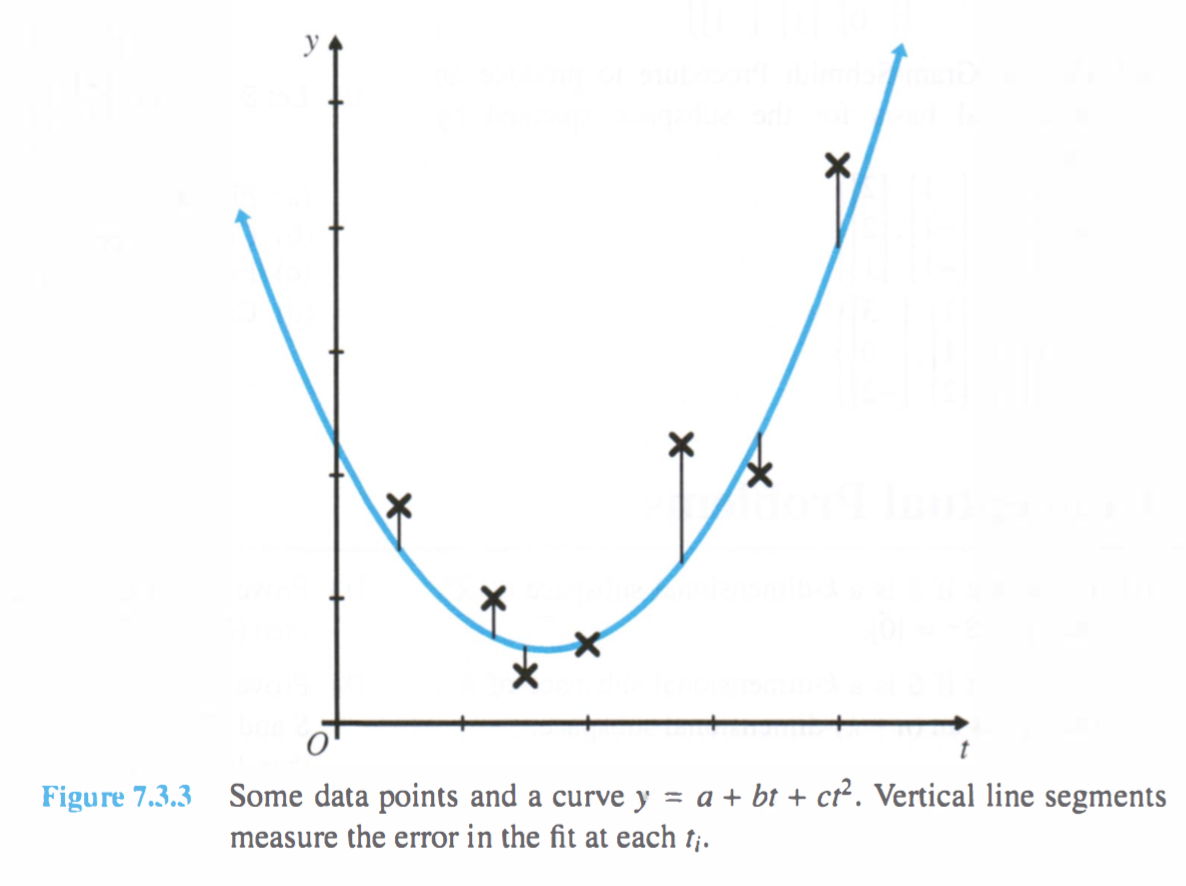
\includegraphics[scale=0.4]{least_squares} \par}

As an \textbf{example}, we'll look at measurements, where the data fits a curve of the form $y = a + bt + ct^2$. Then we will minimize the sum of the squares of the errors:
\begin{equation} \label{7.3-1}
    \begin{split}
        \sum_{n}^{i = 1} e_i^2 = \sum_{n}^{i = 1} (y_i - (a + bt_i + ct_i^2))^2
    \end{split}
\end{equation}

To find the parameters $a, b$ and $c$ that minimize this expression for given values, we will use projections and set up the problem as follows:
\begin{equation} \label{7.3-2}
    \begin{split}
        \|\vec{y}_i - (a\vec{1} + b\vec{t} + c\vec{t}^2)\|^2 = \sum_{n}^{i = 1} (y_i - (a + bt_i + ct_i^2))^2
    \end{split}
\end{equation}

Thus, the problem of finding the curve of best fit is reduced to finding $a, b$ and $c$ such that $a\vec{1} + b\vec{t} + c\vec{t}^2$ is the vector in $\mathbb{S}$ that is closest to $\vec{y}$. By the Approximation Theorem, this vector is $proj_{\mathbb{S}} \vec{y}$.

The \textbf{design matrix} $X$ is then:
\begin{equation} \label{7.3-3}
    \begin{split}
        X = \begin{bmatrix}\vec{1} & \vec{t} & \vec{t}^2\end{bmatrix}
    \end{split}
\end{equation}

Then the error vector can be written as $\vec{e} = \vec{y} - X\vec{a}$ and the \textbf{normal equations} for the least squares fit are
\begin{equation} \label{7.3-4}
    \begin{split}
        X^T (\vec{y} - X\vec{a}) = \vec{0} \> \textrm{, or } \> \vec{a} = (X^T X)^{-1} X^T \vec{y}
    \end{split}
\end{equation}

% -------------------------------------------------- %

\subsubsection{Overdetermined Systems}
Suppose that $A \vec{x} = \vec{b}$ is a system of $p$ equations and $q$ variables, where $p > q$. Furthermore, if the system is inconsistent, there are to many equations to be satisfied. The next best approach is to find a vector $\vec{x}$ that minimizes the ``error'' $\|A \vec{x} = \vec{b}\|$ and solve the consistent system $A \vec{x} = proj_{Col(A)} \vec{x}$:
\begin{equation} \label{7.3-5}
    \begin{split}
        A^T A \vec{x} = A^T \vec{b}
    \end{split}
\end{equation}

% ================================================== %
% == Symmetric Matries and Quadratic Forms  == %
% ================================================== %

\section{Symmetric Matries and Quadratic Forms}

% ================================================== %

\subsection{Diagonalization of Symmetric Matrices [8.1]}

% -------------------------------------------------- %

\subsubsection{Symmetric Properties}
\begin{enumerate}[label=\bfseries (\arabic*)] \itemsep0pt \parskip0pt
    \item An $n \times n$ matrix $A$ is symmetric if and only if $\vec{x} \cdot (A \vec{y}) = (A \vec{x}) \cdot \vec{y}$ for all $\vec{x}, \vec{y} \in \mathbb{R}^n$. In other words: $A^T = A$.
    \item if $\vec{v}_1$ and $\vec{v}_2$ are eigenvectors of a symmetric matrix A corresponding to distinct eigenvalues $\lambda_1$ and $\lambda_2$, then $\vec{v}_1$ is orthogonal to $\vec{v}_2$.
    \item If $A$ is a symmetric matrix, then all eigenvalues of $A$ are real.
\end{enumerate}

% -------------------------------------------------- %

\subsubsection{Orthogonally Diagonalizable}
Every symmetric matrix can be diagonalized, also by an orthogonal matrix. A matrix $A$ is said to be \textbf{orthogonally diagonalizable} if there exists an orthogonal matrix $P$ and a diagonal matrix $D$ such that
\begin{equation} \label{8.1-1}
    \begin{split}
        P^T A P = D
    \end{split}
\end{equation}

% ================================================== %

\subsection{Quadratic Forms [8.2]}
A \textbf{quadratic form} on $\mathbb{R}^n$, with corresponding symmetric matrix $A$, is a function $Q : \mathbb{R}^n \to \mathbb{R}$ defined by
\begin{equation} \label{8.2-1}
    \begin{split}
        Q(\vec{x}) = \sum_{i.j = 1}^{n} a_{ij} x_i x_j = \vec{x}^T A \vec{x}
    \end{split}
\end{equation}

% -------------------------------------------------- %

\subsubsection{Diagonal Form}
A quadratic form $Q(\vec{x})$ is in \textbf{diagonal form} if all the coefficients $a_{jk}$ with $j \neq k$ are equal to $0$. Equivalently, $Q(\vec{x})$ is in diagonal form if its corresponding symmetric matrix is diagonal.

% -------------------------------------------------- %

\subsubsection{Classifications of Quadratic Forms}
\begin{enumerate}[label=\bfseries \arabic*.] \itemsep0pt \parskip0pt
    \item \textbf{Positive definite} if $Q(\vec{x}) > 0$ for all $\vec{x} \neq \vec{0}$
    \item \textbf{Negative definite} if $Q(\vec{x}) < 0$ for all $\vec{x} \neq \vec{0}$
    \item \textbf{Indefinite} if $Q(\vec{x}) > 0$ for some $\vec{x}$ and $Q(\vec{x}) < 0$ for some $\vec{x}$
    \item \textbf{Positive semidefinite} if $Q(\vec{x}) \geq 0$ for all $\vec{x}$
    \item \textbf{Negative semidefinite} if $Q(\vec{x}) \leq 0$ for all $\vec{x}$
\end{enumerate}

% -------------------------------------------------- %

\subsubsection{Symmetric Matrices}
Let $Q(\vec{x}) = \vec{x}^T A \vec{x}$, where $A$ is a symmetric matrix. Then
\begin{enumerate}[label=\bfseries \arabic*.] \itemsep0pt \parskip0pt
    \item $Q(\vec{x})$ is positive definite if and only if all eigenvalues of $A$ are positive
    \item $Q(\vec{x})$ is negative definite if and only if all eigenvalues of $A$ are negative
    \item $Q(\vec{x})$ is indefinite if and only if some of the eigenvalues of $A$ are positive and some are negative
\end{enumerate}

% ================================================== %
% ================================================== %
% ================================================== %
% ================================================== %

% \section{Appendix}
% //todo

\end{multicols*}
\end{document}
